\documentclass[english, 11pt]{article}

\usepackage{notes}
\usepackage{epigraph}
\usepackage{epstopdf}
%\usepackage{paracol}

% Uncomment these for a different family of fonts
% \usepackage{cmbright}
% \renewcommand{\sfdefault}{cmss}
% \renewcommand{\familydefault}{\sfdefault}

%\newcommand{\thiscoursecode}{[XXXX] (\#\#\#)}
\newcommand{\thiscoursename}{Quantum Mechanics}
\newcommand{\thisprof}{Ivan Iorsh}
\newcommand{\me}{Pavel Dmitriev}
\newcommand{\thisterm}{Autumn 2015}
%\newcommand{\website}{MYWEBSITE.COM}

% Headers
\chead{\thiscoursename \ Course Notes}
\lhead{\thisterm}


%%%%%% TITLE %%%%%%
\newcommand{\notefront} {
	\pagenumbering{roman}
	\begin{center}
	
		%{\ttfamily \url{\website}} {\small}
		
		%\textbf{\Huge{\noun{\thiscoursecode}}}{\Huge \par}
		
		{\Huge{\noun{\thiscoursename}}}\\ \vspace{0.1in}
		
		{\noun \thisprof} \ $\bullet$ \ {\noun \thisterm} \ $\bullet$ \ {\noun {ITMO University}} \\
	
	\end{center}
}

\newcommand{\hl}[1]{\textcolor{red}{#1}}


% Begin Document
\begin{document}

	% Notes front
	\notefront
	% Table of Contents and List of Figures
	\tocandfigures
	% Abstract
	\doabstract{Quantum Mechanics Lecture Notes.}
	
	\section{Introduction}
	\subsection{Schr\"odinger formalism}
	
		\begin{equation}
			\hat{f}\Phi =  E \Phi
		\end{equation}
	
		\begin{equation}
			\Phi \rightarrow dP = |\Phi|^2dq
		\end{equation}
		
		\begin{equation}
			x \leftrightarrow \hat{x}
		\end{equation}

		\begin{equation}
			p_x \leftrightarrow -i\hbar \frac{\partial}{\partial x}
		\end{equation}
	
		\begin{equation}
			f \leftrightarrow \hat{f}
		\end{equation}	
		
		\begin{equation}
			\bar{f} = \int \hat{f}dp = \int \Phi^* \hat{f} \Phi dq 
		\end{equation}
	
	\subsection{Heisenberg formalism}
		\epigraph{Schr\"odinger was good at math, which is why his quantum mechanics formalism is full of complex mathematical constructs. Heisenberg, on the other hand, had a lot of difficulty with math, which is why his matrix quantum mechanics formalism is limited almost exclusively to linear algebra constructs}{Roman ... }
	
		\begin{tabular}{c | c | c }
			Name & Schr\"odinger & Heisenberg \\
			\hline
			\hline
			\ &&\\
			
			 State Basis & Wave function of basis states $ \{ \Phi_n \} $ & Column vector of basis states $\begin{pmatrix}\phi_1\\...\\ \phi_n\end{pmatrix}$ \\[3ex]		
			\hline
			\hline
			\ &&\\
			
			Observables & Operator $ \bar{f} = \int \Phi_n^* \hat{f} \Phi_m$ & Operator matrix $\begin{pmatrix}\phi_{11} & ... & \phi_{n1} \\ & ... & \\ \phi_{1n} & ... & \phi_{nn}\end{pmatrix}$ \\[3ex]
			\hline
			\hline
			
			\ &&\\
			Shr\"odinger Equation & $ \hat{f}\Phi =  E \Phi$ & $\begin{pmatrix}\phi_{11} & ... & \phi_{n1} \\ & ... & \\ \phi_{1n} & ... & \phi_{nn}\end{pmatrix} \begin{pmatrix}\psi_1\\...\\ \psi_n\end{pmatrix} = \lambda \begin{pmatrix}\psi_1\\...\\ \psi_n\end{pmatrix}$ \\[3ex]
			\hline
			\hline			
		\end{tabular}
	
		\subsubsection{Building an operator's matrix}
		
	
	\subsection{Pauli uncertainty principle}
		
		\subsubsection{Black holes}
		\subsubsection{Quantum Pencil}
			\cite{easton2007quantum}
		
	\subsection{Problems}
	\section{Analytical Solutions}
	\subsection{Rectangular quantum well}
		\begin{figure}
			\centering
			\begin{tikzpicture}[scale=4,cap=round,>=latex]
	\draw [<->] (-2, 1.5) -- (-2, 0) -- (1.5, 0);
	\node [left] at (-2, 1.5) {$U$};
	\node [below] at (1.5, 0) {$z$};
	
	\draw [line width=1.5] (-2, 1) -- (-1, 1) -- (-1, 0) -- (0, 0) -- (0, 1) -- (1, 1);
	\draw [dashed] (-1, 1) -- (-1, 1.5);
	\draw [dashed] (0, 1) -- (0, 1.5);
	
	\node [left] at (-2, 1) {$U_0$};
	\node [below] at (-1, 0) {$-\frac{d}{2}$};
	\node [below] at (0, 0) {$\frac{d}{2}$};
	
	\node at (-1.5, 1.2) {I};
	\node at (-0.5, 1.2) {II};
	\node at (0.5, 1.2) {III};										
\end{tikzpicture}
			\caption{Finite rectangular quantum well}
		\end{figure}
		
	\subsection{Harmonic oscillator}
	\subsection{Spherically symmetric potential}
	\subsection{Problems}
		\subsubsection{Rectangular quantum well}
			Double quantum well
			
			Double quantum barrier
			
			Minimal transistor size
			
			
	\section{Quasi-classical approximation}
	\subsection{Problems}
		\subsubsection{Exponential potential}
			\begin{figure}[!h]
				\centering
				\begin{tikzpicture}[scale=1,cap=round,>=latex]
\draw [<->] (0, 3) -- (0, 0) -- (7, 0);
\node [left] at (0, 3) {$U$};
\node [below] at (7, 0) {$x$};

\draw [line width=1.5] (0, 0) -- (2, 0) -- (2, 3/2);
\draw[domain=2:7,smooth,line width=1.5, variable=\x] plot ({\x},{3/\x});

\node [below] at (2, 0) {$a$};

\end{tikzpicture}
				\caption{Exponentially decaying potential barrier}
			\end{figure}
			For a potential barrier:
			\begin{align}
				U(x) = \left\{ \begin{aligned}
					0,\quad x < a \\
					\frac{\alpha}{x},\quad x > a
				\end{aligned}
				\right. \\
			\end{align}
			and a particle with $E > 0$, what are the reflection and transmission coefficients?
			
		\subsection{Hemisphere potential}
			\begin{figure}[!h]
				\centering
				\begin{tikzpicture}cap=round,>=latex]
	\begin{axis}[grid=none,
	axis x line=middle,
	axis y line=left,	
	enlargelimits,
	xtick={-1,0,1},
	xticklabels={$-a$, $0$, $a$},
	ytick={1},
	yticklabels={$U_0$},
	domain=-1.2:1.2
	]
	
	\addplot[no markers, line width=1.5, samples=50, domain=-1:1] {cos(deg(pi*x/2))};
	\end{axis}								
\end{tikzpicture}
				\caption{Hemisphere potential barrier}
			\end{figure}
			For a potential barrier:
			\begin{align}
				U(x) = U_0 \cos(\frac{\pi}{2a}x), \quad -a \leq x \leq a
			\end{align}
			and a particle with $E > 0$, what are the reflection and transmission coefficients?
		\subsection{Minimal transistor size}
			\begin{figure}[!h]
				\centering
				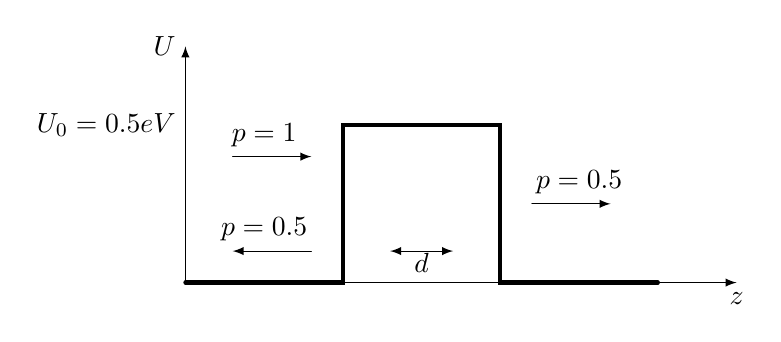
\begin{tikzpicture}[scale=2,cap=round,>=latex]
	\draw [<->] (-2, 1.5) -- (-2, 0) -- (1.5, 0);
	\node [left] at (-2, 1.5) {$U$};
	\node [below] at (1.5, 0) {$z$};
	
	\draw [line width=1.5] (-2, 0) -- (-1, 0) -- (-1, 1) -- (0, 1) -- (0, 0) -- (1, 0);
	
	\node [above] at (-0.5, 0) {$d$};
	\draw [<->] (-0.7, 0.2) -- (-0.3, 0.2);	
	
	\node [left] at (-2, 1) {$U_0 = 0.5\si{eV}$};

	\draw [->] (-1.7, 0.8) -- (-1.2, 0.8);
	\node [above] at (-1.5, 0.8) {$p = 1$};
		
	\draw [<-] (-1.7, 0.2) -- (-1.2, 0.2);
	\node [above] at (-1.5, 0.2) {$p = 0.5$};

	\draw [->] (0.2, 0.5) -- (0.7, 0.5);	
	\node [above] at (0.5, 0.5) {$p = 0.5$};
												
\end{tikzpicture}
				\caption{Model transistor}
			\end{figure}
			
			\begin{align}
				m_{el} \approx& 0.3 m_0 \\
				m_0 \approx& 10^{-30}\si{kg} \\
				p =& |\Psi|^2
			\end{align}			
			
			Calculate the size of a quantum barrier at which an electron's probability of tunneling through is equal to $0.5$ using the quasi-classical approach, and compare it to the exact solution.
		
		\subsection{Classical limit*}	
			For a potential $U(x)$ that possesses a certain number of bound states with energies $E_n$, in the limit $n\rightarrow\infty$, we transition into classical mechanics. 
			
			How does $\Delta E = E_{n+1}-E_n$ change for $n\rightarrow\infty$?
  
	\section{Spin}
	\subsection{Angular momentum}
		\subsubsection{Classical}
			\begin{figure}[!h]
				\centering
				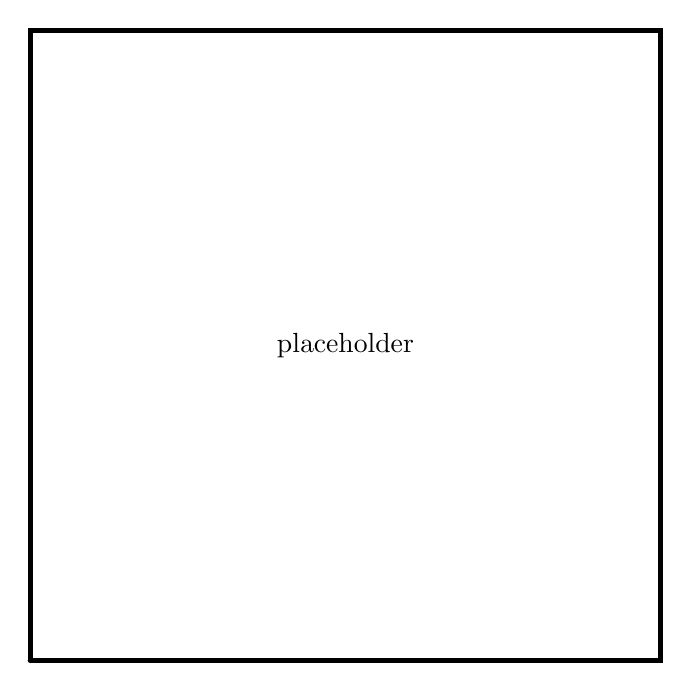
\begin{tikzpicture}[scale=2,cap=round,>=latex]
	\draw [line width=2] (-2, -2) -- (-2, 2) -- (2, 2) -- (2, -2) -- (-2, -2);
	
	\node at (0, 0) {placeholder};
\end{tikzpicture}
				\caption{Classical angular momentum}
				\label{clasmoment}
			\end{figure}
			
			\begin{align}
				\vec{L} =& \vec{r}\times\vec{p} =
				\begin{vmatrix}
					\vec{e_x} & \vec{e_y} & \vec{e_z} \\
					x & y & z \\
					p_x & p_y & p_z \\
				\end{vmatrix} \\
				=& \vec{e_x}(yp_z - zp_y) + \vec{e_y}(zp_x - xp_z) + \vec{e_z}(xp_y - yp_x) \\
				=& \vec{e_x}L_x + \vec{e_y}L_y + \vec{e_z}L_z
			\end{align}
			
			%Building on classical angular momentum is the Rutherford atomic model:
			%\begin{figure}[!h]
			%	\centering
			%	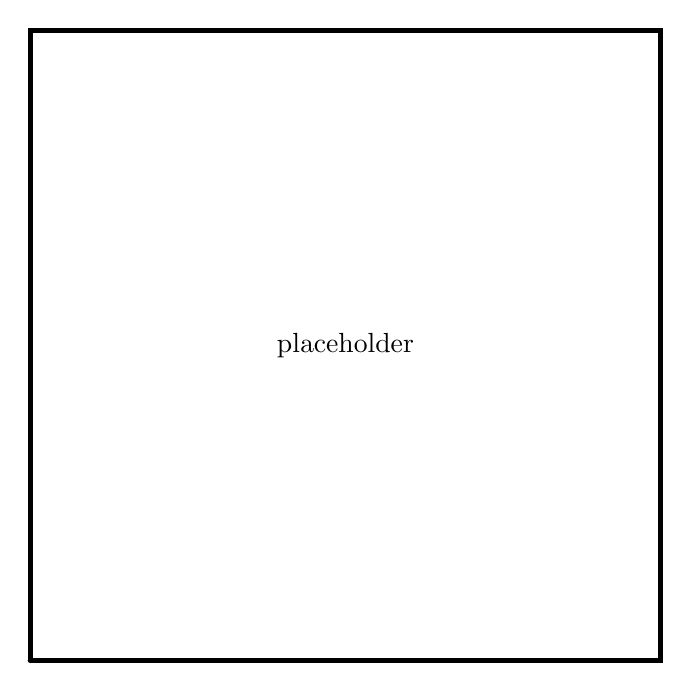
\begin{tikzpicture}[scale=2,cap=round,>=latex]
	\draw [line width=2] (-2, -2) -- (-2, 2) -- (2, 2) -- (2, -2) -- (-2, -2);
	
	\node at (0, 0) {placeholder};
\end{tikzpicture}
			%	\caption{Rutherford atom}
			%	\label{ruthatom}
			%\end{figure}
			%
			%\begin{align}
			%	\frac{mv^2}{r} =& \frac{ke^2}{r^2} \\
			%	m\vec{a} =& \vec{F_c}
			%\end{align}
			%
			%\begin{list}[Problems with the Rutherford model]
			%	\item Discrete energy levels
			%	\item 
			%\end{list}
		\subsubsection{Quantum}
			\begin{align}
				\hat{\vec{p}} =& -i\hbar\vec{\nabla}, \qquad \vec{\nabla} = \vec{e_x}\frac{\partial}{\partial x} + \vec{e_y}\frac{\partial}{\partial y} + \vec{e_z}\frac{\partial}{\partial z} \\
				p_x =& -i\hbar \frac{\partial}{\partial x}, \quad p_y = -i\hbar \frac{\partial}{\partial y}, \quad p_z = -i\hbar \frac{\partial}{\partial z} \\
				\hat{\vec{L}} =& -i\hbar\vec{r}\times\vec{\nabla} \\
				\hat{L_x} =& -i\hbar(y\frac{\partial}{\partial z} - z\frac{\partial}{\partial y}), \quad \hat{L_y} = -i\hbar(z\frac{\partial}{\partial x} - x\frac{\partial}{\partial z}), \quad \hat{L_z} = -i\hbar(y\frac{\partial}{\partial x} - x\frac{\partial}{\partial y}) 
			\end{align}
			
			\hl{Proof!} Commutators:
			\begin{equation}
				\left[\hat{L_x}, \hat{L_y}\right] = i\hbar\hat{L_z}, \quad
				\left[\hat{L_z}, \hat{L_x}\right] = i\hbar\hat{L_y}, \quad
				\left[\hat{L_y}, \hat{L_z}\right] = i\hbar\hat{L_x}
			\end{equation}
			
			Uncertainty: \hl{Wait, what?}
			\begin{align}
				\Delta \hat{L_x} = \hat{L_x} - \left<\hat{L_x} \right>, \quad
				\Delta \hat{L_y} = \hat{L_y} - \left<\hat{L_y} \right>, \quad
				\Delta \hat{L_z} = \hat{L_z} - \left<\hat{L_z} \right> \\
				\left<(\Delta\hat{L_x})^2 \right> = \left<\hat{L_x}^2 \right> - \left<\hat{L_x} \right>^2 \\
				\left<(\Delta\hat{L_y})^2 \right> = \left<\hat{L_y}^2 \right> - \left<\hat{L_y} \right>^2 \\
				\left<\hat{L_x} \right> = \int \Psi^* \hat{L_x} \Psi dV \\ 
				\left<(\Delta\hat{L_x})^2 \right>\left<(\Delta\hat{L_y})^2 \right> \geq \frac{\hbar^2|\left<\hat{L_z}\right>|^2}{4} \\
				\left<(\Delta x)^2 \right>\left<(\Delta p_x)^2 \right> \geq \frac{\hbar^2}{4} \nonumber				
			\end{align}
			
			Generally it isn't possible to measure $L_x, L_y, L_z$ at once. 
		
	\subsection{Problems}    
	\section{Perturbation theory}    
	\subsection{Time-independent}
	\subsection{Time-dependent}
	\subsection{Problems}
	\section{Problem Solutions}
	\subsection{Introduction}
	\subsection{Analytical solutions}
	\subsection{Quasiclassical approximation}
	\subsection{Spin}			
	\subsection{Petrubation theory}				
	
	\newpage
	\phantomsection
	\addcontentsline{toc}{section}{References}
	\bibliographystyle{ieeetr}
	\bibliography{references}
	%%%%%%%%%%%%%%%%%%%%%%%%%%%%%%%%%%%%%%%%%%%%%%%
\end{document}
